\section{OpenAI Gym}
\label{sec:openaigym}
OpenAI \texttt{gym} \cite{1606.01540} is a toolkit for developing and comparing
reinforcement learning algorithms, without making assumptions about the
structure of the agent interacting with the environment, in order to
keep development flexible to updates on both sides.

\subsection{Framework}
The framework of \texttt{gym} allows to interact easily
with an environment, giving the developers to tools they need to perform
actions and to observe the state of the environment itself. In this way it is
possible to focus more on the development of the agent without spending
time on the structure of the world.

\texttt{gym} makes it possible to interact with multiple kinds of environments.
Among these, the authors of the framework developed the support for
Arcade Learning Environment \cite{bellemare13arcade}, which includes all the
classing Atari games, including Breakout, which has been used in this project.

\subsection{Examples}
Let's consider a simple example to understand how \texttt{gym} works and
how the framework can be used to interact with an environment.
The description will follow Algorithm \ref{lst:gym-breakout-example-py}.

\lstinputlisting[caption={Example of a random interaction with the \texttt{gym}
    environment \texttt{BreakoutNoFrameskip-v4}, used also in our experiments
    of subsection \ref{subsec:experiments}.},
    label={lst:gym-breakout-example-py},
    language=Python]{implementation/gym-breakout-example.py}

Initially (line 1) the framework is imported. Then (line 3-4) an environment
is created specifying its name and initializing it. The program makes a
random agent interact randomly with the environment for 1000 timesteps (lines
6-11) before closing the environment. Line 7 renders the current
observation of the environment on screen, line 8-9 performs a random action
between those available in this Brekout version, note that the method
\texttt{step} return an \texttt{observation} (shown in Fig.
\ref{fig:gym-breakout-image-example}), which is an array of pixels
that represent the current state of the environment, a \texttt{reward},
which is a value return by the game after performing the specified action
\texttt{action}, a boolean value \texttt{done}, which is \texttt{True} when
the game is over, \texttt{False} otherwise, and \texttt{info} which contains
extra information about the game. Lines 10-11 handles the case when the game
is over, resetting the environment.

\begin{figure}
    \centering
    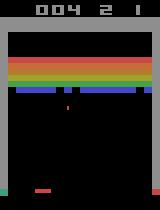
\includegraphics[width=0.3\textwidth]{images/gym-breakout-image-example.jpg}
    \caption{Observation of a frame of the environment
        \texttt{BreakoutNoFrameskip-v4}.}
    \label{fig:gym-breakout-image-example}
\end{figure}
